\chapter{Ergebnisse und Diskussionen}

\section{Ergebnisse aus den Versuchen}

\subsection{Generierte Fragebögen}
%((15 +30 + 50 +100 + 150 + 300) * 2) =
Da insgesammt 1.290 Fragen generiert werden lassen sich diese aufgrund des zeitlichen Aufwandes nicht alle bewerten. Aus jedem Fragebogen werden stichprobenartig 10 Fragen ausgesucht und überprüft, wie Sinnvoll diese sind.

\subsubsection{Deepseek/Nomic}

Bei der generierung von Fragen mit DeepSeekkam es zu mehreren Problemen.\\
Bei dem Fragenset welches 300 Fragen umfassen sollte traten Folgende Probleme auf.
\begin{itemize}
    \item Von den angeforderten 300 Fragen wurden nur 267 Fragen (11 \%) überhaupt generiert, der Rest ist aufgrund von technischen Problemen oder ungültigen Antworten seitens DeepSeek nicht generiert worden
    \item Von diesen sind 101 zu Themen rund um Bezahlmethoden, Versand und ähnliches. In den Dokumenten welche dem DeepSeek zu verfügung gestellt wurden traten diese Themen nicht auf. Diese Fragen sind daher als ungültig bewertet worden.
\end{itemize}

Am Ende bleiben also 166 von 300 Fragen übrig, \textbf{ca. 45 \%} der angeforderten Fragen sind nicht daher irrelevant!

Beim generieren des Testsets mit 100 Fragen sah das ganze etwas besser aus
\begin{itemize}
    \item Von den 100 angeforderten Fragen wurden 88 Fragen generiert. Ganze 12 \% wurden hier auch nicht generiert.
    \item Dieses Mal sind jedoch nur 4 Fragen zu irrelevanten Themen wie Bezahlmethoden, Versand etc.,
\end{itemize}
Am Ende haben wir für das testset mit 100Fragen eine Fehlerquote von \textbf{16 \%}.

Aus der Tabelle 5.1 wird ersichtlich, dass die Fehlerrate in den Testsets für die 400 Dokumente deutlich großer ist. Der Grund dafür wird noch untersucht.

\begin{table}[htbp]
    \centering
    \begin{tabular}{|c|c|c|c|c|}
        \hline
        \textbf{Angefragt} & \textbf{Generiert} & \textbf{Irrelevant} & \textbf{Verlust} & \textbf{Fehlerrate} \\
        \hline
        15   & 11  & 0   & 4  & 27 \% \\
        30   & 27  & 7   & 3  & 33 \% \\
        50   & 40  & 0   & 10 & 20 \% \\
        100  & 88  & 4   & 12 & 16 \% \\
        150  & 137 & 49  & 13 & 41 \% \\
        300  & 267 & 101 & 33 & 45 \% \\
        \hline
    \end{tabular}
    \caption{Übersicht der generierten Fragen und Fehlerraten pro Testset für DeepSeek}
\end{table}


\subsubsection{Open-AI}


\begin{table}[htbp]
    \centering
    \begin{tabular}{|c|c|c|c|c|}
        \hline
        \textbf{Angefragt} & \textbf{Generiert} & \textbf{Irrelevant} & \textbf{Verlust} & \textbf{Fehlerrate} \\
        \hline
        15   & 12   & 0   & 3  & 20\% \\
        30   & 30   & 1   & 0  & 3\%  \\
        50   & 48   & 0   & 2  & 4\%  \\
        100  & 95   & 1   & 5  & 6\%  \\
        150  & 150  & 8   & 0  & 5\%  \\
        300  & 300  & 16  & 0  & 5\%  \\
        \hline
    \end{tabular}
    \caption{Übersicht der generierten Fragen und Fehlerraten pro Testset}
\end{table}

\subsection{Manuelle Auswertung der Fragebögen}
\subsubsection{DeepSeek}

Bei der manuellen Sichtung der Testsets wurden weitere Fehler entdeckt

Neben dem vorhin angesprochenen Problem mit den irrelevanten Themen hat DeepSeek auch zwischendurch Fragen und beispielhafte Antworten auf Englisch generiert.

Frage:
How much does it cost?

Antwort:
For orders under \$50, shipping costs \$5.99.

Bei dieser Frage hat das LLM verdreht, wer bezahlt und fragt, wie viel die Schulen weniger \textbf{verdienen} und nicht wie viel sie weniger \textbf{bezahlen}.

Frage:
Hallo! Ich bin Schulleiter/in und überlege, ob wir als Pilotenschule bei Develop 4 Future teilnehmen sollen. Könnt ihr mir sagen, wie viel weniger die beiden Pilotenschulen im ersten Jahr verdienen verglichen mit anderen Schulen?

Antwort:
Die beiden Pilotenschulen verdienen im ersten Jahr 2.000 \texteuro weniger als die anderen Schulen.

Auch gab es Probleme mit Fragen, die zu allgemein gefasst waren. \"Ich möchte wissen, wie die Verfügbarkeit der Webseite für Schulen ist.\"
Hier ist nicht geklärt, worauf sich die Verfügbarkeit bezieht. Es könnte sich hier sowohl um die Frage handeln, ob aktuell eine Webseite gekauft werden kann oder auch wie viel Prozent Erreichbarkeit garantiert wird.

Ebenso ist "Wie hoch ist die Gesamtsumme der Passiva?" eine Frage welche nicht spezifiziert um welches Jahr es sich handelt Fehleranfällig.

Es gab auch Fragen, welche sich vom Kontext verwirren lassen haben.\\
Frage:\\
Hallo, ich bin ein kanadischer Student, der sich für die Schulsysteme in Deutschland interessiert. Könntest du mir erklären, warum sich die meisten Grundschulen in NRW befinden?\\
Antwort:\\
Die meisten Grundschulen befinden sich in NRW, damit sie das vom Bundesland zur Verfügung gestellte System Logineo einbinden können, das Lehrer- und Schülerverwaltung bietet.

\begin{table}[htbp]
    \centering
    \begin{tabular}{|l|c|}
        \hline
        \textbf{Testset} & \textbf{Fragliche Fragen} \\
        \hline
        Ollama – 10 Dok (10)   & 2 \\
        Ollama – 10 Dok (30)   & 6 \\
        \hline
        \multicolumn{2}{|l|}{\textbf{Summe 10 Dok: \quad 8 / 20 = 40\%}} \\
        \hline
        Ollama – 100 Dok (50)  & 2 \\
        Ollama – 100 Dok (100) & 4 \\
        \hline
        \multicolumn{2}{|l|}{\textbf{Summe 100 Dok: \quad 6 / 20 = 30\%}} \\
        \hline
        Ollama – 400 Dok (150) & 5 \\
        Ollama – 400 Dok (300) & 8 \\
        \hline
        \multicolumn{2}{|l|}{\textbf{Summe 400 Dok: \quad 13 / 20 = 65\%}} \\
        \hline
        \multicolumn{2}{|l|}{\textbf{Gesamt (Ollama): \quad 27 / 60 = 45\%}} \\
        \hline
    \end{tabular}
    \caption{Anzahl fraglicher Fragen pro Testset und Gesamtübersicht für Ollama}
\end{table}

Die Fehlerqute von 45\% zeigt, dass die fragen die DeepSeek generiert nicht einfach eingesetzt werden können. 
Es sind hier eindeutige Unterschiede im Vergleich zu von Menschen generierten Fragen erkenntlich.

\subsubsection{OpenAI}

Bei ChatGPT wurden auch Mängel bei der manuellen Überprüfung festgestellt. \\
Die Fragen werden so gestellt, dass sie den ``gegebenen Kontext'' bewerten sollen. Es fehlen dadurch wichtige Infromationen welche zum finden der relevanten Dokumente fehlen.\\
``Analysieren Sie den bereitgestellten Kontext und erläutern Sie unter der Voraussetzung, dass Sie keine externen Quellen verwenden dürfen, welches zentrale Thema oder welcher Hauptzweck in dem Textabschnitt behandelt wird. Begründen Sie Ihre Antwort anhand spezifischer Textstellen.''

Bei einer Frage war das vorliegende dokument ein Fragebogen, Fehlerhafterweise wurde die erste Option als die richtige Antwort verstanden, da der Fragebogen nicht ausgefüllt ist ergibt dies keinen Sinn.

Auch eine Frage welche die Antwort schon beinhaltet wurde generiert:
``Kannst du mir erklären, was das besondere Merkmal des neuen Schulwebseiten Systems ist, das ich als Lehrer verwenden werde, um Abwesenheitsmeldungen schnell und einfach zu veröffentlichen?''

\begin{table}[htbp]
    \centering
    \begin{tabular}{|l|c|}
        \hline
        \textbf{Testset} & \textbf{Fragliche Fragen} \\
        \hline
        OpenAi – 10 Dok (10)   & 0 \\
        OpenAi – 10 Dok (30)   & 3 \\
        \hline
        \multicolumn{2}{|l|}{\textbf{Summe 10 Dok: \quad 3 / 20 = 15\%}} \\
        \hline
        OpenAi – 100 Dok (50)  & 3 \\
        OpenAi – 100 Dok (100) & 1 \\
        \hline
        \multicolumn{2}{|l|}{\textbf{Summe 100 Dok: \quad 4 / 20 = 20\%}} \\
        \hline
        OpenAi – 400 Dok (150) & 5 \\
        OpenAi – 400 Dok (300) & 7 \\
        \hline
        \multicolumn{2}{|l|}{\textbf{Summe 400 Dok: \quad 12 / 20 = 60\%}} \\
        \hline
        \multicolumn{2}{|l|}{\textbf{Gesamt (OpenAi): \quad 19 / 60 = 31{,}67\%}} \\
        \hline
    \end{tabular}
    \caption{Anzahl fraglicher Fragen pro Testset und Gesamtübersicht für OpenAi}
\end{table}

Wenn wir die Testsets mit Code (150/300 Fragen) ignorieren kommen wir auf eine Fehlerquote von 17,5 \%, dies ist die Hälfte von Ollamas 35 \% also eine deutliche Verbesserung jedoch immer noch eine beachtliche Menge!

Bei einem Vergleich mit einem von Menschen erstellten Fragebogen sind hier jedoch deutlichen Unterscheide was die Qualität der Fragen betrifft.


\subsection{Auswertung der Reports}
Für die Auswertung der Reports werden wieder die selben Fragen wie vorher aus den Testsets verwenden.
Dabei wird geguckt

\begin{itemize}
    \item Ist die Frage an sich richtig? Das heißt, ergibt es Sinn mit dem ursprünglich gegebenen Kontext diese Frage zu stellen.
    \item Wurde die Frage vom RAG richtig beantwortet
    \item Ist die Bewertung der vier Metriken richtig?
    \item Auffällig war, dass Answere Relevancy am häufigsten abweichend war, deswegen wurd hier zusätzlich Bewertet ob die Bewertung besser oder schlechter sein sollte.
\end{itemize}

\subsubsection{Manuelle Auswertung DeepSeek}
Bei der Manuellen Bewertung fällt auf, dass ganze 64 \% nicht richtig beantwortet wurden, dabei muss jedoch beachtet werden, dass 43 \% erst garnicht als sinnvoll sind.

Auch die nicht bewerteten Metriken sind mit bis zu 83 \% fast unbrauchbar, dies liegt wieder daran, dass das LLM zu lange zum Antworten braucht oder eine ungültige Antwort geliefert hat.
% Tabelle für DeepSeek
\begin{table}[h!]
    \centering
    \begin{tabular}{|l|c|c|c|}
    \hline
    \textbf{Metrik} & \textbf{Richtig} & \textbf{Falsch} & \textbf{Nicht bewertet} \\
    \hline
    Richtige Frage                        & 34 (56.7\%) & 26 (43.3\%) & -- \\
    Gültige Antwort                       & 22 (36.7\%) & 38 (63.3\%) & -- \\
    context\_precision                    & 10 (16.7\%) & --         & 50 (83.3\%) \\
    faithfulness                          & 11 (18.6\%) & 2 (3.4\%)  & 47 (78.0\%) \\
    context\_recall                       & 60 (100\%)  & --         & -- \\
    answer\_relevancy                     & 43 (71.7\%) & 15 (25.0\%) & 2 (3.3\%) \\
    answer\_relevancy sollte höher sein  & 4 (100\%)   & --         & -- \\
    \hline
    \end{tabular}
    \caption{Verteilung der Bewertungen für DeepSeek (mit Prozentangaben)}
\end{table}


\subsubsection{Manuelle Auswertung OpenAI}
Bei der Nutzunge der OpenAi Api für GPT-4 kam es zu keinen Timeouts oder ähnlichem welche zu ungültigen Werte führen würden. Es kam jedoch zu zwischenzeitlichen RateLimits, diese könnten von einer Firma jedoch bei einem Vertragsschluss mit OpenAI erhöht werden.

% Tabelle für OpenAI
\begin{table}[h!]
    \centering
    \begin{tabular}{|l|c|c|}
    \hline
    \textbf{Metrik} & \textbf{Richtig} & \textbf{Falsch} \\
    \hline
    Richtige Frage                        & 43 (72.9\%) & 16 (27.1\%) \\
    Gültige Antwort                       & 42 (71.2\%) & 17 (28.8\%) \\
    context\_precision                    & 56 (94.9\%) & 3 (5.1\%) \\
    faithfulness                          & 51 (86.4\%) & 8 (13.6\%) \\
    context\_recall                       & 57 (96.6\%) & 2 (3.4\%) \\
    answer\_relevancy                     & 43 (72.9\%) & 16 (27.1\%) \\
    answer\_relevancy sollte höher sein  & 7 (53.8\%)  & 6 (46.2\%) \\
    \hline
    \end{tabular}
    \caption{Verteilung der Bewertungen für OpenAI (gesamt) mit Prozentangaben}
\end{table}

GPT-4.1 schneidet deutlich besser als DeepSeek ab, 27 \% an nicht sinnvollen Fragen ist jedoch immer noch ein hoher Wert!
Die hälfte der ungültigen Antworten ist durch sinnlose Fragen bedingt, hier ziehen sich also die schlecht generierten Fragen durch.


\subsubsection{Probleme mit Code}
Da es sowhol bei der Testset generierung als auch bei der Bewertung der Testsets, die 400 Dokumente nutzten, höhere Fehlerraten zu beobachten sind wird das genauer untersucht.

\begin{figure}[htbp]
    \centering
    \begin{minipage}[b]{0.48\textwidth}
        \centering
        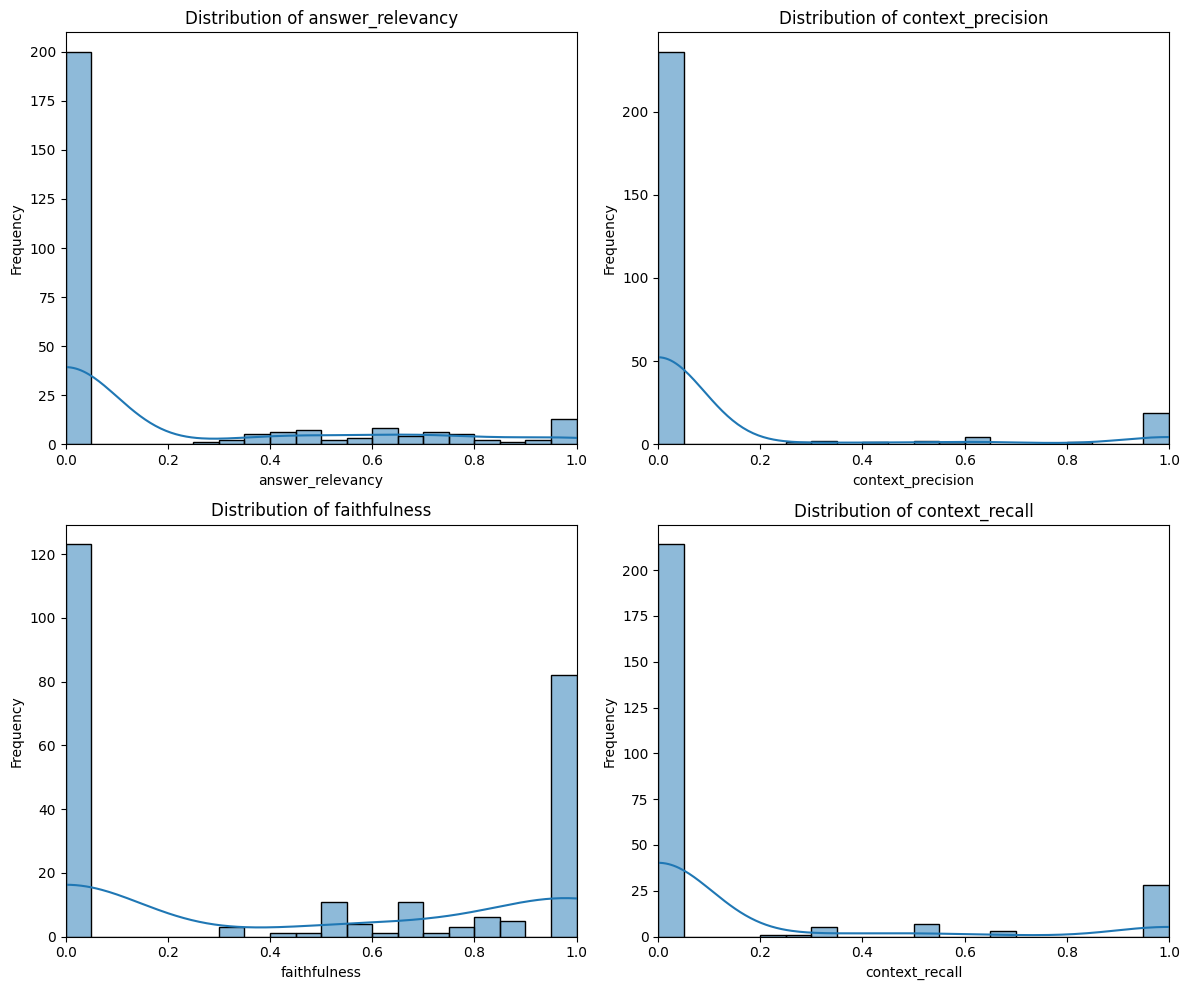
\includegraphics[width=\textwidth]{images/3_3_code_invest_D_D.png}
        \caption{DeepSeek Ergebnis für 300 Fragen}
        \label{fig:deepseek}
    \end{minipage}
    \hfill
    \begin{minipage}[b]{0.48\textwidth}
        \centering
        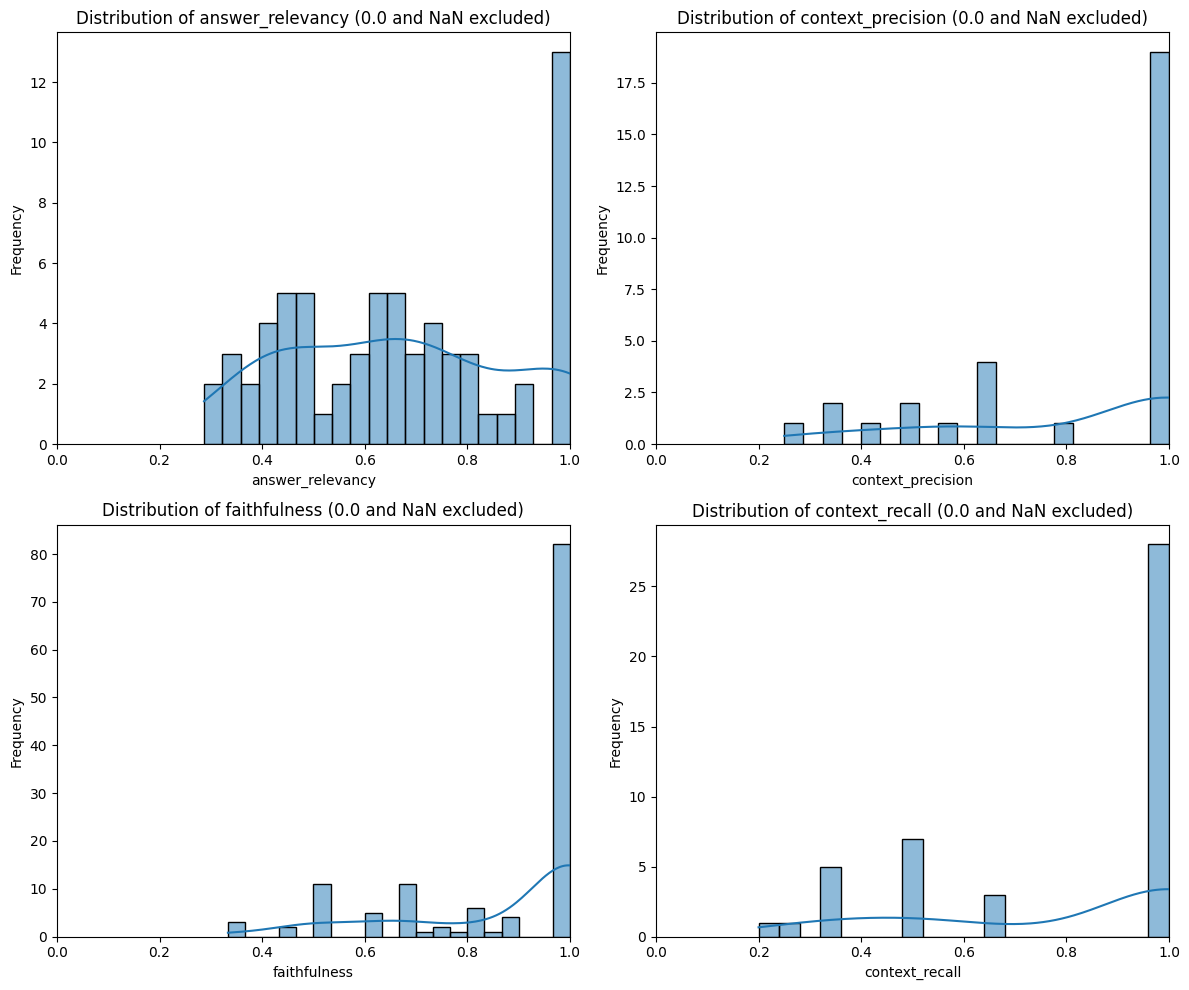
\includegraphics[width=\textwidth]{images/127_44_code_invest_O_O.png}
        \caption{ChatGPT Ergebnis für 300 Fragen}
        \label{fig:chatgpt}
    \end{minipage}
\end{figure}
Der Vergleich der Anzahl der 0.0 Bewertungen mit DeepSeek (Abbildung 5.1) im Vergleich zu OpenAI (Abbildung 5.2) ist eindeutig.\\

106 (~40 \%) der Ergebnisse insgesamt 276 zu bewertenden Fragen waren mit komplett 0.0 bewertet worden. Bei der Analyse der Speziellen Charaktere im Kontextes fällt auf, dass 89 Bewertungen (~83 \%) zu mehr als 5 \% nur aus diesen besteht, dies deutet darauf hin, dass DeepSeek starke Probleme hat Fragen mit Code zu generieren und oder zu finden.
\begin{figure}[htbp]
    \centering
    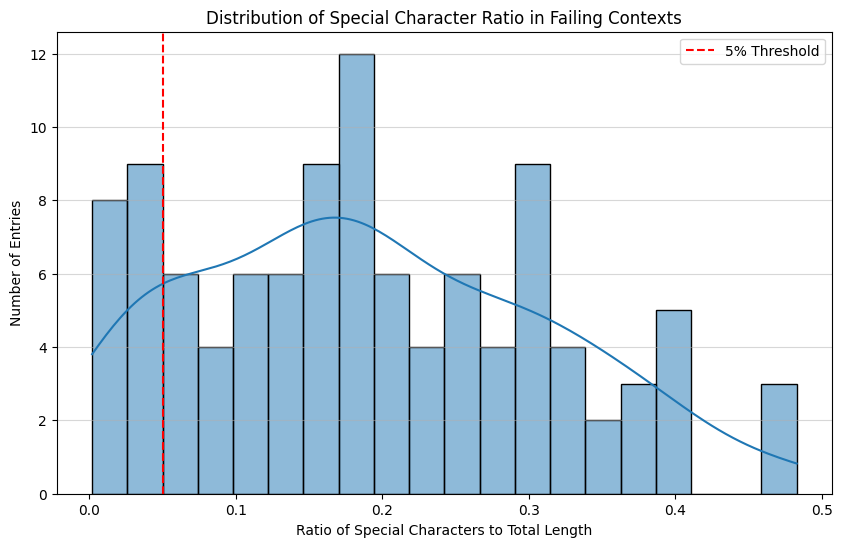
\includegraphics[width=0.8\textwidth]{images/3_3_special_characters.png}
    \caption{Abweichungen des Faithfullness Scores.}
    \label{fig:sample-image}
\end{figure}

Ein großer Teil der Fragen hat sich also durch Dokumente mit minderer Qualität, im Bezug auf mögliche Fragestellungen, verwirren lassen.
es zeigt sich wieder einmal, dass die Qualität der Daten eine entscheidende Rolle spielt!
Wenn wir uns jetzt die Ergebnisse ohne Dokumente welche Code enthalten angucken sehen wir, dass die 0.0 Bewertungen bei DeepSeek deutlich zurück gehen aber wie zu erwarten OpenAi\'s ChatGPT-4 immer noch deutlich besser ist.

\begin{figure}[htbp]
    \centering
    \begin{minipage}[b]{0.48\textwidth}
        \centering
        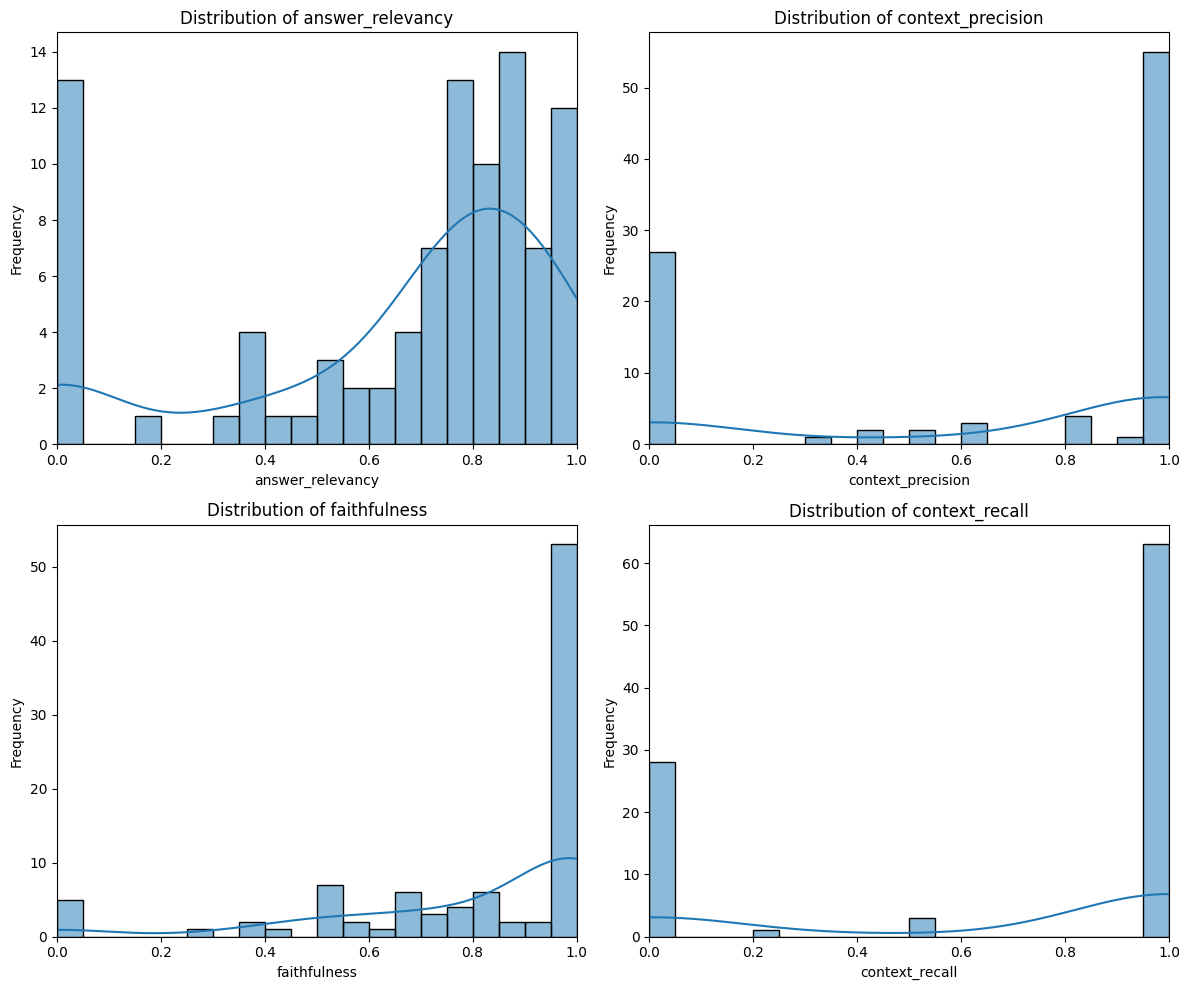
\includegraphics[width=\textwidth]{images/20_4_D_D_distribution.png}
        \caption{DeepSeek Ergebnis für 100 Fragen}
        \label{fig:deepseek}
    \end{minipage}
    \hfill
    \begin{minipage}[b]{0.48\textwidth}
        \centering
        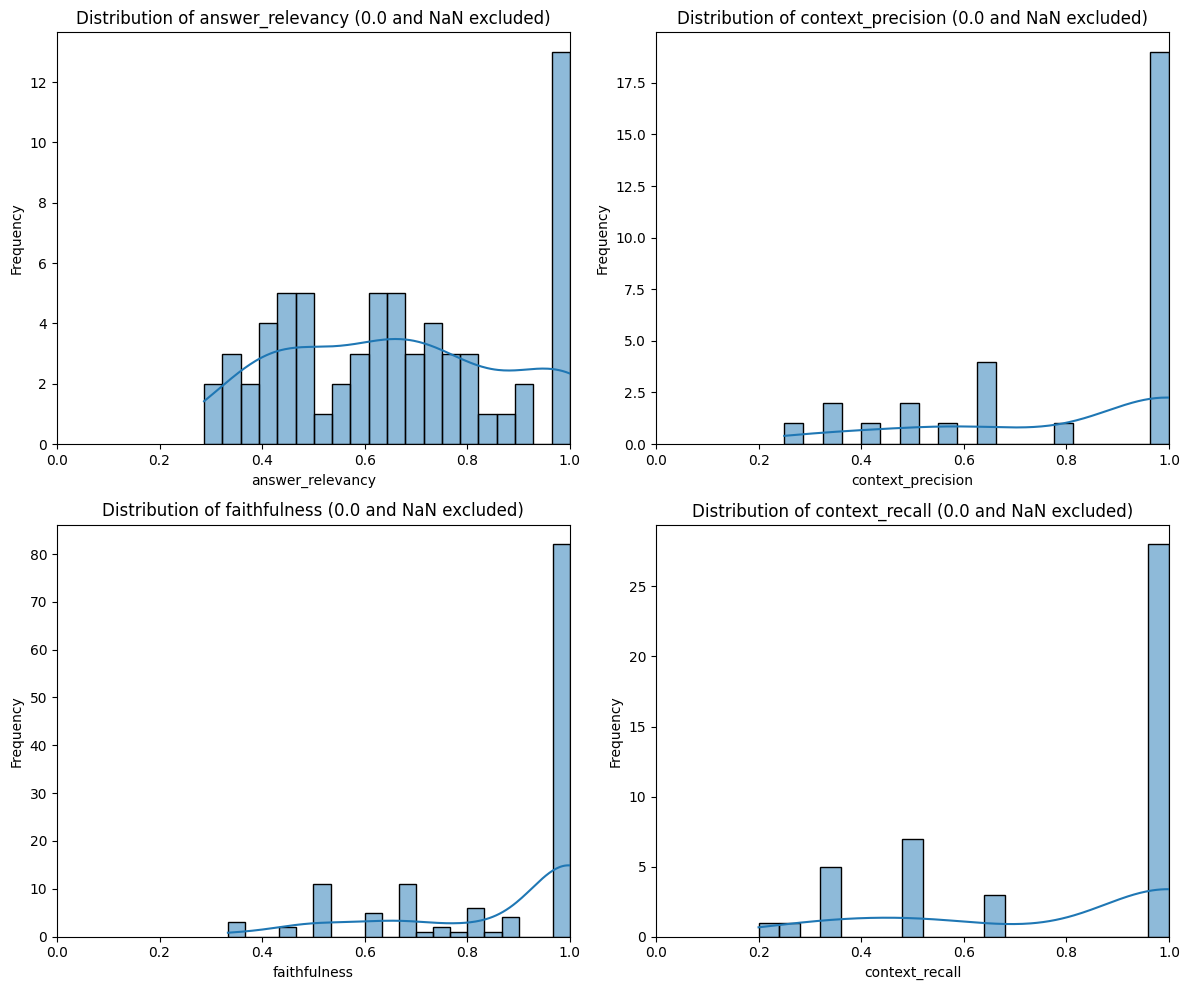
\includegraphics[width=\textwidth]{images/127_38_O_O_distribution.png}
        \caption{ChatGPT Ergebnis für 100 Fragen}
        \label{fig:chatgpt}
    \end{minipage}
\end{figure}


\subsection{Unterschiede über mehrere Durchläufe}

Um zu gucken, wie sich die Ergebnisse von Durchlauf zu Durchlauf unterscheiden wurden für das Testset mit 100 Fragen für 100 Dokumente mit beiden Modellen vier Durchläufe vorgenommen.
In diesem Versuch geht es, um die Unterscheide pro Durchlauf für das Modell festzustellen und nicht die Modelle miteinander zu vergleichen.

\begin{figure}[htbp]
    \centering
    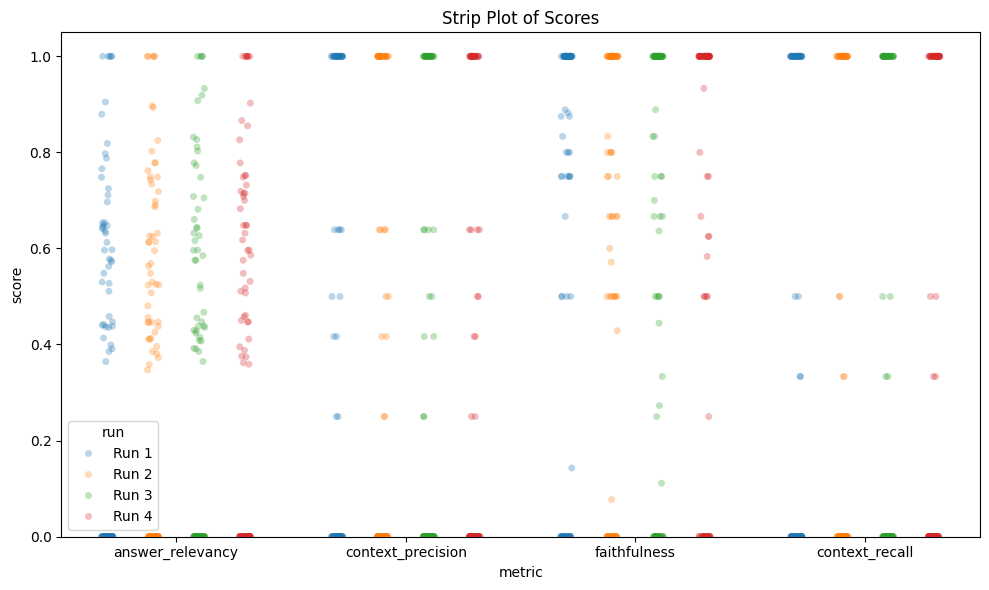
\includegraphics[width=0.9\textwidth]{images/strip_plot_100_100_D_D.png}
    \caption{Bewertung der vier Durchläufe mit DeepSeek}
    \label{fig:sample-image}
\end{figure}

\begin{figure}[htbp]
    \centering
    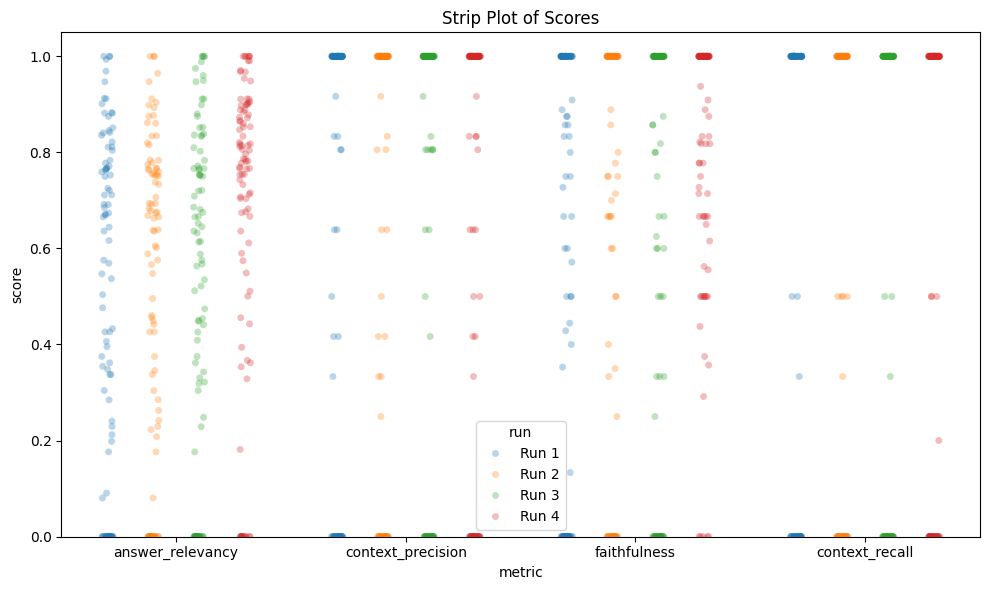
\includegraphics[width=0.9\textwidth]{images/strip_plot_100_100_O_O.png}
    \caption{Bewertung der vier Durchläufe mit GPT-4}
    \label{fig:sample-image}
\end{figure}

Beim Betrachten der Strip Plots lässt sich gut sehen, dass die Verteilung der Werte pro Durchlauf sehr ähnlich sind und keine großen Abweichungen erkennbar sind.

\begin{table}[h!]
    \centering
    \resizebox{\textwidth}{!}{%
    \begin{tabular}{|l|c|c|c|c|c|c|c|c|}
    \hline
    \textbf{Metrik} & \textbf{Mean 1} & \textbf{Mean 2} & \textbf{Mean 3} & \textbf{Mean 4} & \textbf{Std 1} & \textbf{Std 2} & \textbf{Std 3} & \textbf{Std 4} \\
    \hline
    Answer Relevancy    & 0.336 & 0.366 & 0.329 & 0.358 & 0.346 & 0.340 & 0.347 & 0.361 \\
    Faithfulness         & 0.624 & 0.593 & 0.627 & 0.623 & 0.442 & 0.429 & 0.436 & 0.453 \\
    Context Precision    & 0.344 & 0.344 & 0.344 & 0.344 & 0.449 & 0.449 & 0.449 & 0.449 \\
    Context Recall       & 0.415 & 0.415 & 0.415 & 0.415 & 0.484 & 0.484 & 0.484 & 0.484 \\
    \hline
    \end{tabular}%
    }
    \caption{Durchschnittswerte und Standardabweichungen der Metriken über vier Durchläufe für DeepSeek}
\end{table}

Beim Betrachten des Durchschnitts und der Standardabweichung lässt sich für die answer relevancy und die faithfullnes sehen, dass eine gewisse Schwankung vorhanden ist, die Metriken für den Kontext sind jedoch sehr konstant!
Bei der answer relevancy lässt sich ein Unterschied von 3.7 \% feststellen, bei der faithfullnes 3.1 \%, dies liegt für 4 Durchläufe im Rahmen bedeutet aber auch, dass dies beim Einrichten einer automatischen Pipeline berücksichtigt werden sollte.

\begin{table}[h!]
    \centering
    \resizebox{\textwidth}{!}{%
    \begin{tabular}{|l|c|c|c|c|c|c|c|c|}
    \hline
    \textbf{Metrik} & \textbf{Mean 1} & \textbf{Mean 2} & \textbf{Mean 3} & \textbf{Mean 4} & \textbf{Std 1} & \textbf{Std 2} & \textbf{Std 3} & \textbf{Std 4} \\
    \hline
    Answer Relevancy    & 0.490 & 0.493 & 0.666 & 0.681 & 0.340 & 0.351 & 0.315 & 0.314 \\
    Faithfulness         & 0.632 & 0.613 & 0.815 & 0.800 & 0.434 & 0.444 & 0.273 & 0.295 \\
    Context Precision    & 0.669 & 0.684 & 0.666 & 0.670 & 0.445 & 0.445 & 0.444 & 0.445 \\
    Context Recall       & 0.663 & 0.667 & 0.681 & 0.671 & 0.461 & 0.466 & 0.458 & 0.456 \\
    \hline
    \end{tabular}%
    }
    \caption{Durchschnittswerte und Standardabweichungen der Metriken über vier Durchläufe für GPT-4}
\end{table}


\subsection{Zuverlässigkeit von Metriken}

Um genauer zu untersuchen, wie sich die Metriken bei merhfacher ausführung verhalten wurden die vier Metriken jeweils 50 Mal ausgeführt.
Bei der bewertung wurde immer GPT-4.1 verwendet.

\subsubsection{Context Precision\&Recall}
%a5abd219-ea65-4c50-bc33-14f0e36cb19c

%'question': 'Wie viele Schulen können im Moment monatlich ein System ohne Komplikationen eingerichtet bekommen, und welche Faktoren beeinflussen diese Anzahl?',
%'response': 'Im Moment können ohne Komplikationen 10 Schulen pro Monat ein System eingerichtet bekommen. Die Faktoren, die diese Anzahl beeinflussen, umfassen:\n\n1. **Modular System**: ermöglicht Skalierung und zukünftige Erweiterungen.\n2. **Supportprozesse**: Schools müssen Benutzer definieren und bei Fragen Kontakt aufnehmen;.future tutorials könnten den Setup vereinfachen.\n3. **Anpassungsanfragen**: unterschiedliche Wünsche können Ressourcen beanspruchen und Komplexität hervorrufen.\n4. **Stärke des Fördervereins**: Ein starker Förderverein erleichtert Vertrieb und Implementierung.\n\nDiese Faktoren zusammen bestimmen die derzeitige Kapazität von 10 Schulen pro Monat.','retrieved_contexts': ['verleihen dem Produkt den Feinschliff. Dies ist der momentane Stand. Im Verlaufe der nächsten fünf Jahre kann zu einem späteren Zeitpunkt das System so weit erweitert werden, dass Funktionen für weiterführende Schulen eingebracht werden. Dies ist einzig und allein durch das Modular aufgebaute System möglich.',
%Kontext:
%'Aktuell können ohne Komplikationen 10 Schulen pro Monat ein System eingerichtet bekommen. Das Einrichten des Servers ist nur der Anfang in der Zusammenarbeit mit den Grundschulen. Es müssen von der Schule noch die Benutzer festgelegt werden und die jeweiligen Personen melden sich bei Unklarheiten oder Fragen bei Develop 4 Future. Diese Fragen werden in der Zukunft weniger und es wird möglich sein, Tutorials für die häufigsten Fragen zu erstellen.',
%'Es besteht die Gefahr, dass eine Schule sich eine Änderung wünscht, welche nicht mit den Wünschen einer anderen Schule zu vereinbaren sind. Für diesen Fall muss eine Möglichkeit geschaffen werden, beide Funktionen einzubauen und dabei die Komplexität dieser Funktion minimal zu halten. Die Kosten für eine solche Änderung, die sich auf bis zu 1.000 € belaufen können werden direkt an den Kunden weitergegeben, der diese Änderung anfragt.',
%'Je stärker der Förderverein der Grundschulen ist, desto einfacher lässt sich das Produkt inklusive weiterer Verbesserungen verkaufen.\n\n\n\nWenn die Schule das System kaufen möchte, dann ist sind in der Regel die Schulleitung und der Förderverein beteiligt. Weitere LehrerInnen, die vorher an der Webseite gearbeitet haben oder zukünftig daran arbeiten sollen, können auch involviert sein, um Feedback für die Schulleitung und den Förderverein zu geben.'],

Beide Metriken wurden 50 Mal bewertet und haben sich wie bei DeepSeek in der gesamt Bewertung als sehr stabil herausgestellt.


\subsubsection{Answere Relevency}
Hier wurden minimale Abweichungen festgestellt, diese belaufen sich aber auf die zweite Nachkommastelle in der Prozentangabe und sind daher vernachlässigbar

\begin{figure}[htbp]
    \centering
    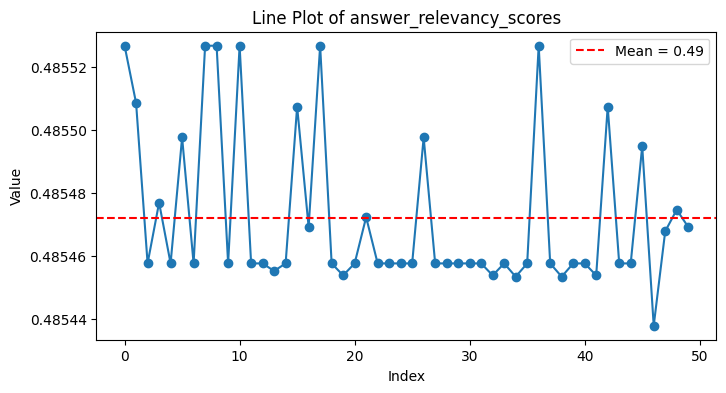
\includegraphics[width=0.8\textwidth]{images/answer_relevancy.png}
    \caption{Abweichungen des Answere Relevancy Scores.}
    \label{fig:sample-image}
\end{figure}

\subsubsection{Faithfullness}
%a5abd219-ea65-4c50-bc33-14f0e36cb19c
Bei der Faithfullness sieht dies schon etwas anders aus. Die richtige Bewertung wäre 62.5 \%, in 66 \% der Fälle war dem auch so, es ist jedoch ersichtlich, dass der Wert Teilweise bis zu 12.5\% abweichen kann.

\begin{figure}[htbp]
    \centering
    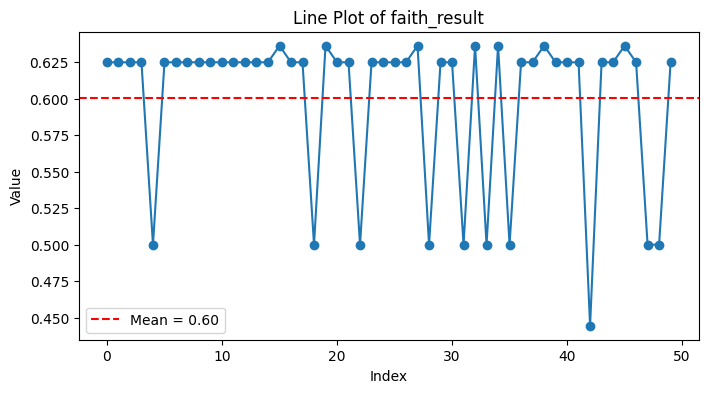
\includegraphics[width=0.8\textwidth]{images/faithfullness.png}
    \caption{Abweichungen des Faithfullness Scores.}
    \label{fig:sample-image}
\end{figure}

Die Faithfullness Metrik hat die größten Schwankungen, dies war auch schon bei dem Versuch mit mehreren Durchläufen ersichtlich.



\subsubsection{Ausführungszeiten DeepSeek}
Da es bei OpenAi zu den Rate Limits kommen kann wurde die Anzahl an gleichzeitigen Abfragen von 16 auf 1 reduziert, da sonst besonders bei längeren durchläufen zu Problemen kommt.
Das führt zu einer deutlichen verschlechterung der Ausführungszeit, bei dem Testset mit 15 Fragen sind wir von 2 Minuten mit maximal 16 gleichzeitigen Anfragen auf 7 Minuten bei maximal einer gleichzeitigen Anfrage.
Mit diesen Zahlen lässt sich annehmen, dass der Versuch mit 300 Fragen ohne Rate Limit seitens OpenAi sicherlich unter einer Stunde geschafft werden könnte.

\begin{table}[h!]
    \centering
    \begin{tabular}{|c|c|}
    \hline
    \textbf{Anzahl} & \textbf{Dauer (hh:mm)} \\
    \hline
    15   & 00:02 \\
    30   & 00:03 \\
    50   & 00:04 \\
    100  & 00:07 \\
    150  & 01:37 \\
    300  & 02:30 \\
    \hline
    \end{tabular}
    \caption{Dauer der Evaluation pro Dokumentenzahl mit OpenAI}
\end{table}

\subsubsection{Ausführungszeiten OpenAi}
Für die Bewertung das Testset mit 300 Fragen (400 Dokumente) wurde Tracing genutzt, die lässt uns genauer gucken, warum gewisse Bewertungen fehlgeschlagen sind.\\ 
Es kam insgesamt zu 20 Fehlern, 12 Zeitüberschreitungen, weil das LLM nicht inerhalb von 10 Minuten geantwortet hat, acht Antworten waren in einem ungültigen Format, sieben davon für context\_recal und eine für faithfullnes.\\
Mit den 20 fehlgeschlagen Metriken kommen wir auf eine Fehlerrate von 1.9 \%.
% 20/(4*267) eig 300 aber die wurden nicht alle generiert
\begin{table}[h!]
    \centering
    \begin{tabular}{|c|c|}
    \hline
    \textbf{Anzahl} & \textbf{Dauer (hh:mm)} \\
    \hline
    15   & 00:41 \\
    30   & 01:03 \\
    50   & 01:35 \\
    100  & 03:41 \\
    150  & 05:20 \\
    300  & 17:29 \\
    \hline
    \end{tabular}
    \caption{Dauer der Evaluation pro Dokumentenzahl}
\end{table}

\subsection{Kostenberechnung}

Die Bewertung des RAGs, mit den 300 Fragen, hat 2 Stunden und 30 Minuten gedauert, dabei sind Kosten in Höhe von 12 Euro entstanden.


Dies kann man mit einer Bewertung, wie in den Versuchen, auf einem Mac Studio (M2 Ultra) vergleichen.
\begin{itemize}
    \item Laufzeit pro Bewertung: 17\,h
    \item Stromkosten: 0{,}12\texteuro/h $\Rightarrow$ 17\,h $\times$ 0{,}12\texteuro/h = \textbf{2{,}04\texteuro}
    \item OpenAI API-Kosten pro Bewertung: 12{,}00\texteuro\\
          Davon sollen 2{,}00\texteuro lokal durch eigene Ausführung ersetzt werden $\Rightarrow$ verbleibende Abschreibung: \textbf{10{,}00\texteuro/Run}
    \item Geräteanschaffung: 7.200\texteuro $\Rightarrow$ amortisiert über 720 Runs à 10{,}00\texteuro
    \item Gesamtkosten pro Run: 2{,}04\texteuro (Strom) + 10{,}00\texteuro (Abschreibung) = \textbf{12{,}04\texteuro}
    \item Gesamtlaufzeit (720 Runs): 720 $\times$ 17\,h = 12.240\,h $\approx$ \textbf{1 Jahr, 4 Monate, 10 Tage}
\end{itemize}



\section{Abhängigkeit der Metriken untereinander}
Dadurch, dass die Metriken für den Kontext einen früheren Schritt in der Abfrage an ein RAG bewerten als die für die Antwort, ergeben sich gewisse Abhängigkeiten.\\


\begin{figure}[htbp]
    \centering
    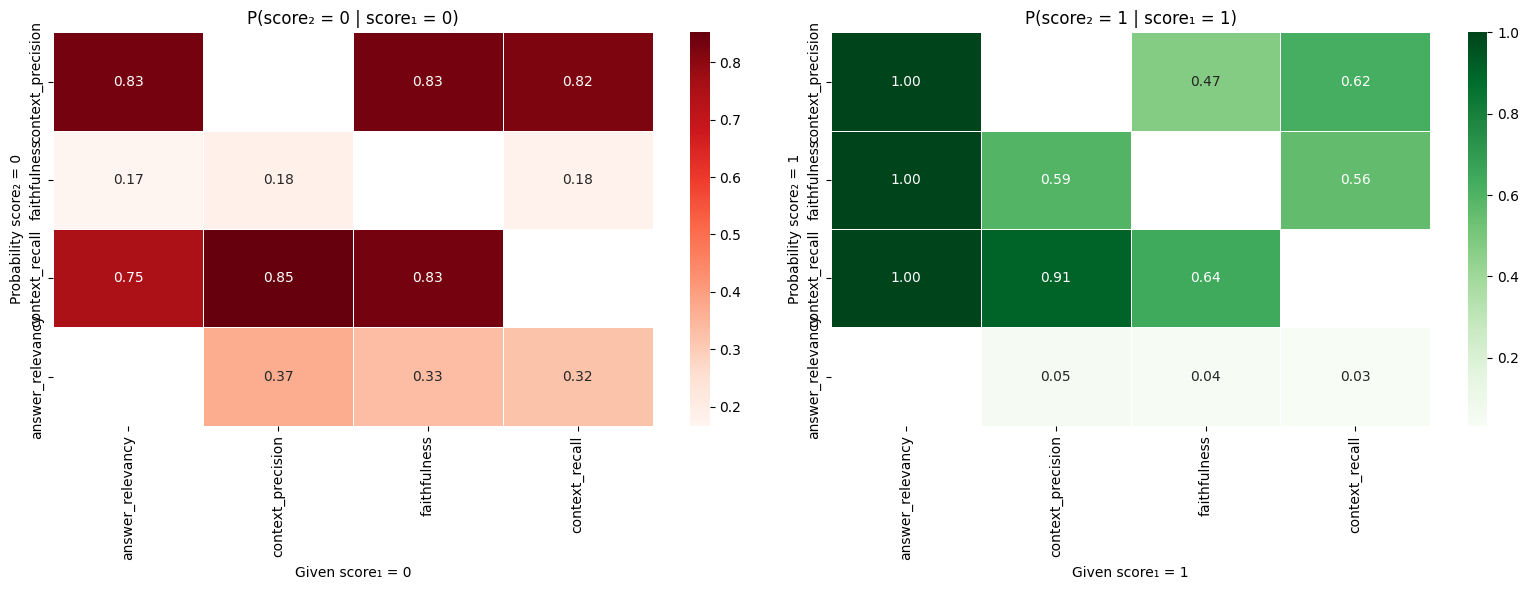
\includegraphics[width=0.8\textwidth]{images/metric_influence_400_300_O_O.png}
    \caption{Abweichungen des Answere Relevancy Scores.}
    \label{fig:sample-image}
\end{figure}

Wenn die Metriken für den Kontext (context\_precision und context\_recall) eine Bewertung von 0 haben ist die Wahrscheinlichkeit, dass die anderen Metriken auch 0 sind relativ hoch.\\
In diesem konkreten Beispiel werden die Abhängigkeiten von dem OpenAI Rag für die 300 Fragen gezeigt, es lässt sich sehen, die faithfullness deutlich weniger von 




\section{Identifikation von Interessenten}

